% Бүлэг 1

\chapter{Хичээлийн хуудас веб системийн судалгаа} % Бүлгийн нэр
\label{Chapter1} % Энэ бүлэг рүү ишлэл хийх бол \ref{Chapter1} командыг ашигла 

%-------------------------------------------------------------------------------

% Агуулгад ашигласан хэвшүүлэлтийн зарим командын тодорхойлолт
\newcommand{\keyword}[1]{\textbf{#1}}
\newcommand{\tabhead}[1]{\textbf{#1}}
\newcommand{\code}[1]{\texttt{#1}}
\newcommand{\file}[1]{\texttt{\bfseries#1}}
\newcommand{\option}[1]{\texttt{\itshape#1}}

%------------------------------------------------------------------------------
\section{Зорилго}
\hspace{1cm}Их сургуулийн оюутан, багш, сургалтын албаны ажилтанд зориулсан хичээлийн хуудас үүсгэж ажиллах, суралцах боломжийг хөнгөвчилнө.
%------------

%-------------------------------------------------------------------------------
\subsection{Системийг хөгжүүлэх үндэслэл}
\hspace{1cm}Сүүлийн жилүүдэд техник технологи, цахим сүлжээ, интернет холбоо хурдацтай хөгжихийн хэрээр сошиал медиаг хүмүүс маш ихээр ашиглаж ажил үүрэг, албан хэргээ зохицуулж, бусадтай харилцах харилцаа хялбарчилж байгаа билээ. Тиймээс яг ийм орчинг их сургуулийн оюутан, багш, ажилчдад бүрдүүлэхэд болохгүй зүйл байхгүй юм.

%-------------------------------------------------------------------------------
\subsection{Системийн цар хүрээ}
\begin{itemize}
	\item Уг системийг их дээд сургуулийн оюутан залуус, эрдэмтэн багш нар хэрэгцээтэй мэдээлэл авах болон солилцох, үйл ажиллагаагаа хялбарчлах зорилгоор ашиглана.
	\item Хичээлийн хуудас гэсэн модул нь багш оюутныг илүү ойртон ажиллах нөхцлийг бүрдүүлнэ.
\end{itemize}

%-------------------------------------------------------------------------------
\subsection{Шинэлэг тал}
\begin{itemize}
	\item Одоогоор бид сошиал медиа гэхээр фейсбүүк, твиттер, ви чат гэх зэрэг бүх нийтийг хамарсан том сүлжээг л мэдэхээс биш яг их сургуулийн хүрээнд ажиллах сошиал сүлжээ тэр бүр байхгүй байгаа юм.
	\item Их сургуулийн сошиал сүлжээ нь тухайн сургуулийн үйл ажиллагааны идэвхитэй, ирээдүйд хөгжих боломжийг нь бүрдүүлнэ.
\end{itemize}

%-------------------------------------------------------------------------------
\newpage
\section{Төстэй системийн судалгаа}
\hspace{1cm}Одоогоор их дээд сургуулиудад хувийн сошиал сүлжээ гэхээсээ илүү фейсбүүк групп болон багш нарын хувийн блог илүү ашиглагдаж байна. Тиймээс эмх цэгцтэй нэгдсэн систем байх шаардлагатай байгаа юм. Тухайн системтэй төстэй дараах веб системүүд байна. 
\begin{itemize}
	\item www.Facebook.com
	\item alison.com
	\item moodle
	\item unimis 
	
\end{itemize}
\subsection{Ижил төстэй монгол систем}
\hspace{1cm}moodle, unimis гэсэн системүүд нь оюутан бүртгэл үүсгэн багш нарын тавьсан мэдээлэл, сорил явын оноо гэх мэт дүнгийн мэдээлэл болон цаашлаад хичээл сонголт зэрэг үйлдлүүдийг л хийх боломжтой байдаг. 

\begin{figure}[htbp]
	\centering
	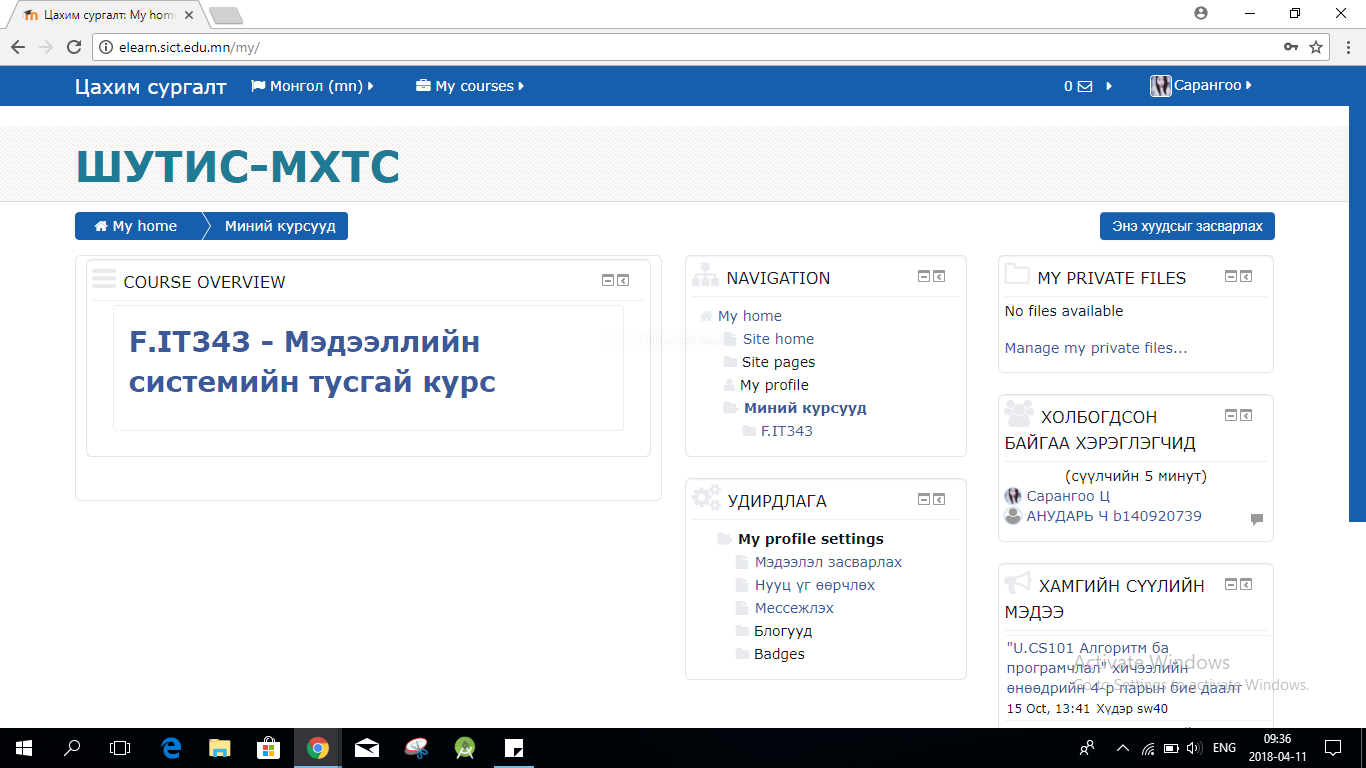
\includegraphics[scale=0.4]{Chart/Capture2}
	\caption[Мүүдл систем]{elearn.sict.edu.mn}
	\label{fig:Capture2}
\end{figure}

\begin{figure}[htbp]
	\centering
	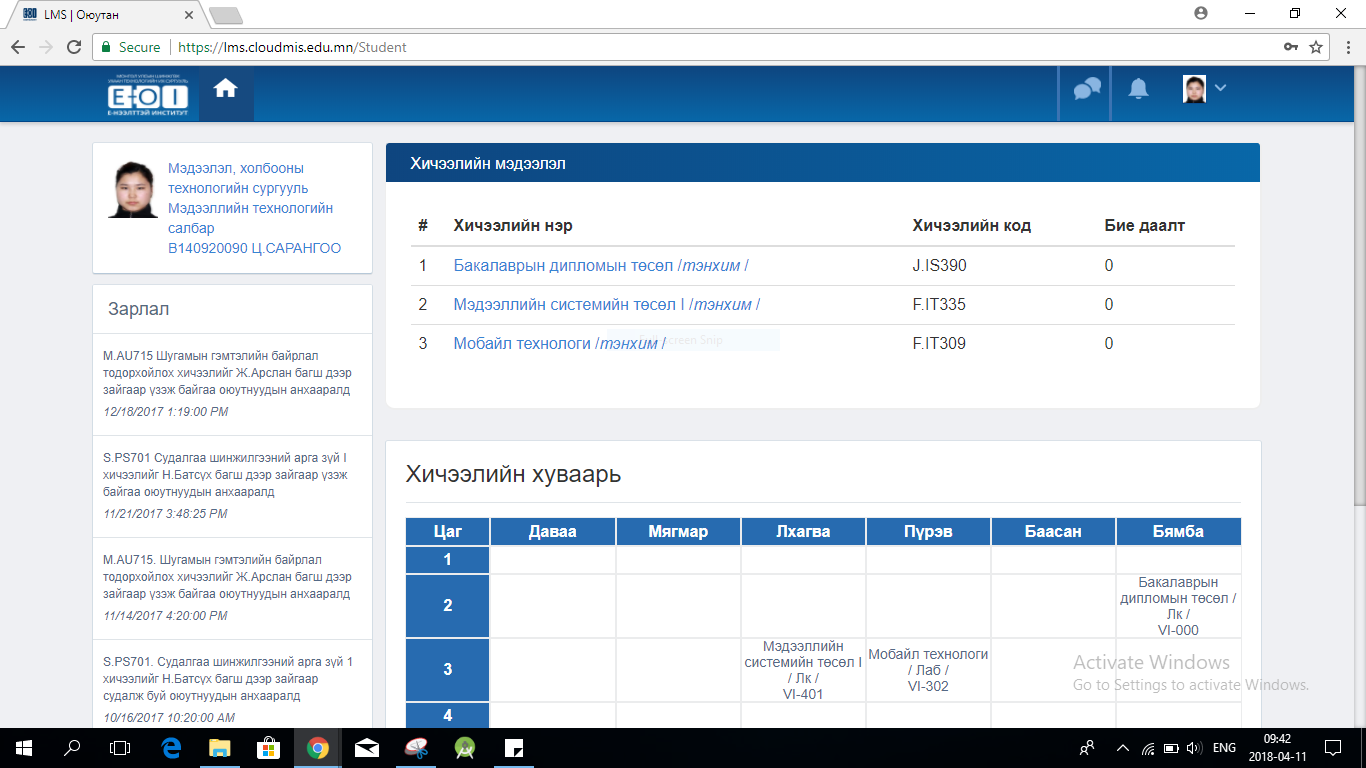
\includegraphics[scale=0.4]{Chart/Capture4}
	\caption[Юнимис систем]{lms.cloudmis.edu.mn}
	\label{fig:Capture4}
\end{figure}
\newpage
\subsection{Ижил төстэй гадаад систем}
Алисоны тухай\\
\hspace{1cm}Алисон нь Дипломын болон Сертификатын түвшинд үнэгүй онлайн курс бэлтгэдэг. Алисон бол хамгийн анхны онлайн үнэгүй сургалтын платформ бөгөөд түүнийг өргөтгөх тогтвортой бие даасан санхүүжилтийн загварыг боловсруулж, ашиглаж байна. Газарзүйн байрлал, эдийн засгийн статус зэрэг бэрхшээлүүдийг үл харгалзан үнэ төлбөргүй боловсрол олгох зорилготойгоор Алисон 1000 үнэгүй онлайн курс, долоо хоног бүр шинэ шинэ саналуудыг оруулдаг. Одоогийн байдлаар тус платформ нь 12 сая гаруй бүртгэгдсэн суралцагч, 1.5 сая төгсөгчидтэй, 175 гаруй мянган хүн үнэгүй сургалтанд хамрагдаж байна. 

\begin{figure}[htbp]
	\centering
	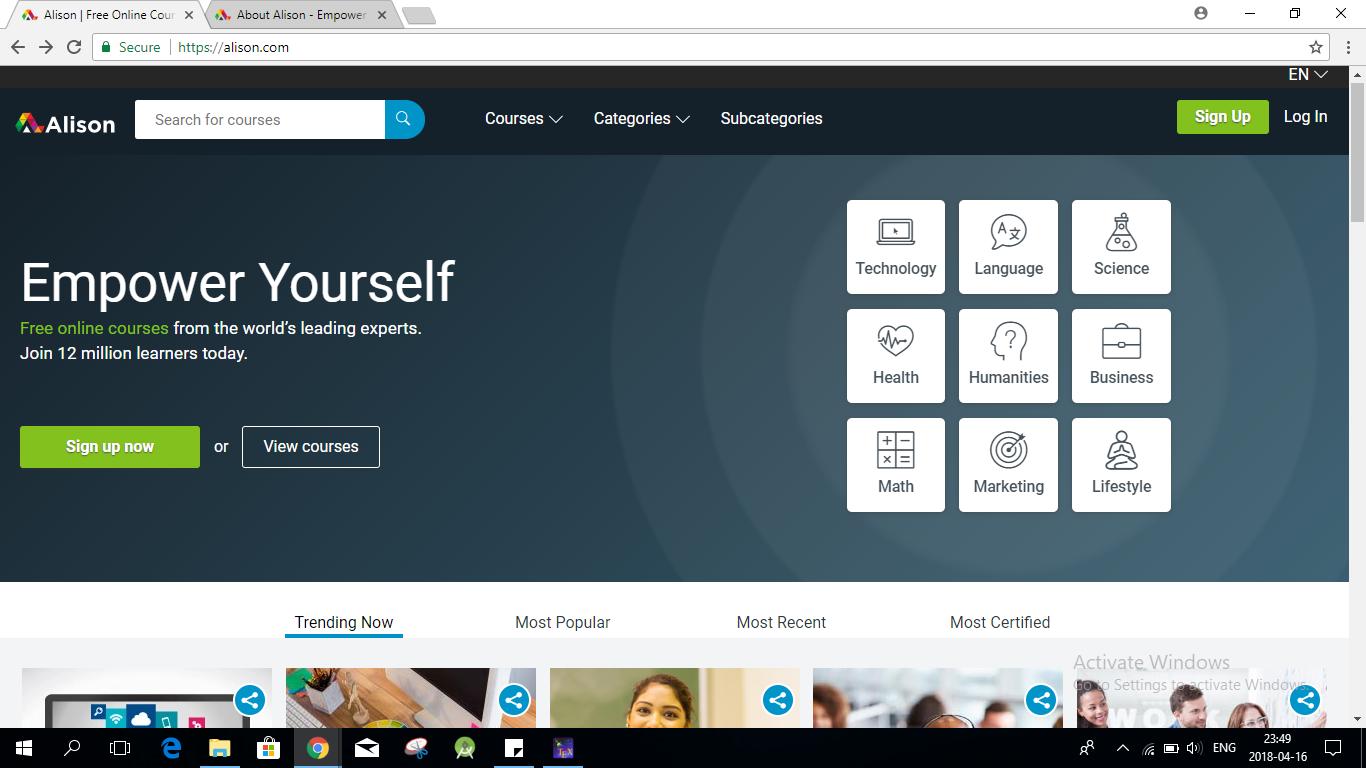
\includegraphics[scale=0.4]{Chart/Capture5}
	\caption[Хичээлийн хуудас судалгаа]{alison.com}
	\label{fig:Capture5}
\end{figure}
\begin{figure}[htbp]
	\centering
	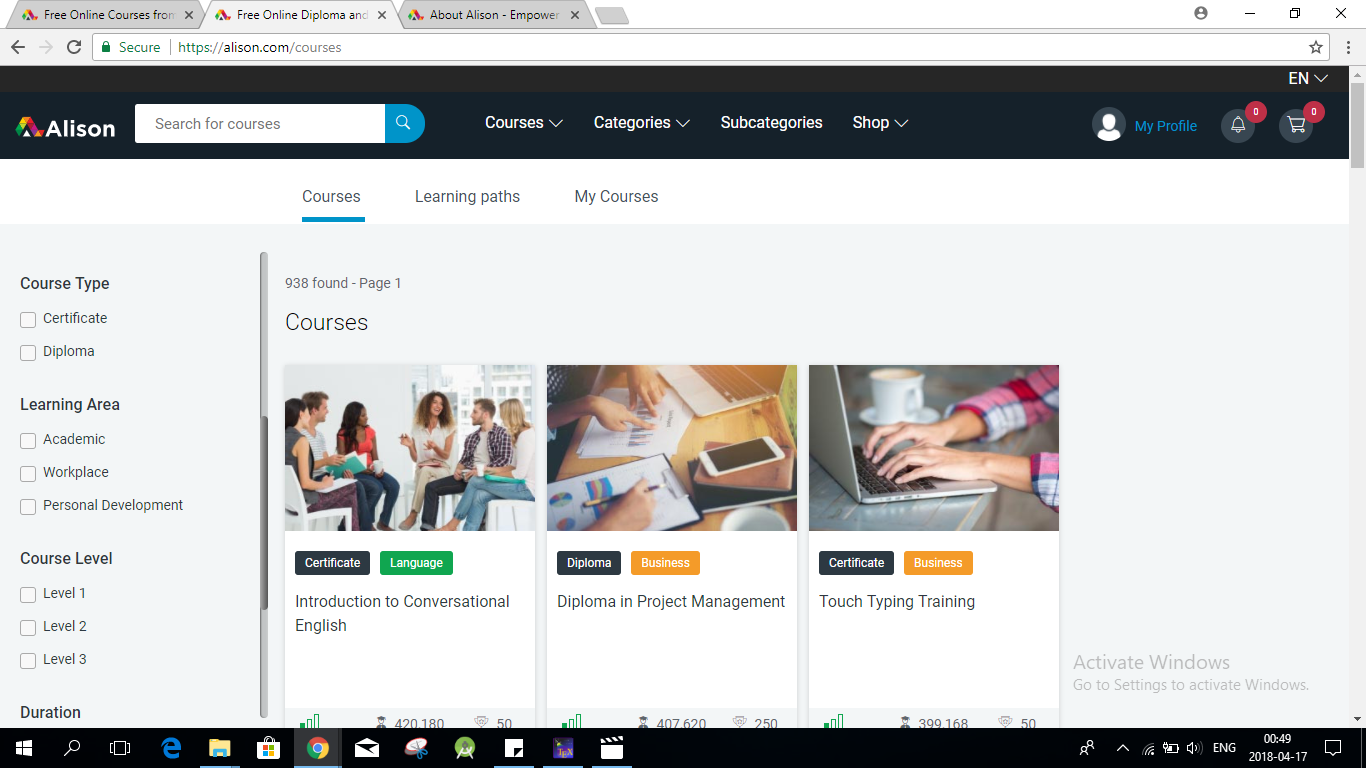
\includegraphics[scale=0.4]{Chart/Capture6}
	\caption[Хичээлийн хуудас судалгаа]{alison.com}
	\label{fig:Capture6}
\end{figure}
\newpage
\section{Технологийн судалгаа}
\subsection{Model View Controller(MVC) архитектур}
\hspace{1cm}Модел-Харагдац-Удирдлага(MVC) нь ПХ-ийн архитектур бөгөөд объект хандлагат ПХ-ийн инженерчлэлд ашиглагддаг архитектур загвар юм. Энэхүү загвар нь бизнес логикийг дэлгэцийн зохиомжоос тусгаарласнаар тест болон хөгжүүлэлтийн дараа арчилгаа тордолгоо хийхэд тус тусад нь хөгжүүлэх боломж олгоно.
\begin{itemize}
	\item Модел (Model) нь мэдээллийг удирдах эсвэл мэдээлэл өөрчлөхөд observer-үүдийг анхааруулахад ашиглагдана.
	\item Харагдац (View) гэдэг нь моделийг хувиргаж харагдах байдалд шилжүүлснийг хэлнэ, ихэвчлэн дэлгэцийн харагдах байдал байна. Хэд хэдэн харагдах байдал нь ганцхан моделийг өөр өөр зорилгоор ашигласан байж болно.
	\item Удирдлага (Controller) нь оролтуудыг хүлээн аваад моделийг дуудаж хариу буцаах үйлдлийг бэлдэнэ. Удирдлага нь оролтуудыг зөвшөөрч тэрхүү оролтууд дээр үндэслэгдсэн үйлдлүүдийг моделийн тусламжтайгаар боловсруулах үүрэгтэй.
\end{itemize}
\subsection{MySQL}
\hspace{1cm}MySQL нь холбоост өгөгдлийн санг удирдах систем юм. MySQL хэмээх нэрний хувьд уг системийг санаачлан хөгжүүлэгч Micheal Widenius-ын охины нэр My + SQL(Structed Query Language) гэсэн утгатай ажээ.
Энэ систем нь GNU (General Public License) буюу нээлтэй эхийн систем учир хүссэн хэн бүхэн хөгжүүлэлтэнд оролцож, үнэгүй хэрэглэж болох юм. Эзэмшигч нь алдарт Java-г хөгжүүлсэн Sun MicroSystems компани байсан ба, одоогоор Sun-г Oracle корпораци эзэмших болсон билээ.
Үнэгүй програм хангамжийн өгөгдлийн санг удирдах системд ихэвчлэн MySQL-ийг хэрэглэдэг бөгөөд тэдгээрийн сонгодог жишээ гэвэл Joomla, Drupal, Wordpress, phpBB гэх мэт агуулга удирдах системүүд (CMS-Content Management System), Wikipedia, Facebook, Google гэх мэт томоохон компаниуд хэрэглэдэг юм.
Хөгжүүлэлт нь C/C++ хэл дээр хийгдсэн ба AIX, BSDi, FreeBSD, HP-UX, i5/OS, Linux, Mac OS X, NetBSD, Novell NetWare, OpenBSD, OpenSolaris, eComStation, OS/2 Warp, QNX, IRIX, Solaris, Symbian, SunOS, SCO OpenServer, SCO UnixWare, Sanos, Tru64, Microsoft Windows гэсэн олон үйлдлийн системүүд дээр ажилладаг.
MySQL бол хамгийн өргөн хэрэглээтэй нээлттэй эхийн (Open Source) өгөгдлийн сан удирдах програм юм. Анх 1995 онд зах зээлд гарсан ба с/с++ хэл дээр бичигдсэн. Одоогийн байдлаар 5.7 нь хамгийн сүүлийн хувилбар болон гараад байна. Энэ сүүлийн хувилбар дээр нэмэгдсэн давуу талууд гэвэл 3 дахин хурдан үйл ажиллагаатай болсон мөн натив JSON дэмжигчтэй болсон гэх мэт шинэлэг үйлдлүүд нэмэгдсэн байна.

\subsection{Php}
\hspace{1cm}Rasmus Lerdorf WWW-д вэб хуудас үүсгэх үедээ өгөгдөл боловсруулах хялбархан арга хайж байгаад 1995 онд PHP хэлийг скрипт хэл байдлаар зохиосон.
PHP нь сервер талын скрипт хэл ба динамик вэб хуудас хийхэд илүү тохиромжтой. Энэ скрипт хэл нь энгийн хэрэглээний вэб сайтаас эхлээд байгууллагын иж бүрэн вэб программ хийж болохоор MySQL мэтийн өгөгдлийн сантай харилцан ажиллах боломжтой.
Хуудас ачаалах үед броузерээр нэг бүрчлэн уншдаг HTML-тэй адилгүй, PHP баримтыг бэлтгэхдээ серверээр урьдчилан боловсруулдаг. PHP код агуулсан хуудас нь хэрэглэгчийн броузерт илгээгдхээс өмнө серверээр боловсруулагдсан байдаг.
PHP хэлний өөр нэг давуу тал бол скриптэн хэл юм. Ихэнх програмчлалын хэлнүүдэд ажиллахын өмнө машины хэл рүү хөрвүүлэх тусгай файлууд /compile/ шаардлагатай байдаг бол PHP хэлний хувьд хөрвүүлэлт хийх шаардлагагүй байдаг тул код засварлах болон шалгахад илүү хурдан байдаг

\subsection{JQuery}
\hspace{1cm}2006 оны эхээр АНУ-ын Нью-Иорк хотын BarCamp-д John Resig хэмээх вэб хөгжүүлэгч залуу jQuery сангийн тухай анх мэдэгджээ. Resig өөрийн вэб сайтдаа: Тухайн үед байгаа сангуудад сэтгэл дундуур байгаагаа, мөн түүнчлэн JavaScript – ий тухай бичилтийг нь багасгаснаар маш их ажил хөнгөвчлөх боломжтой, энгийн үйлдлүүдэд зориулан тусгай хэрэгслүүд нэмэх хэрэгтэй гэж дурдсан байдаг.
Хөгжүүлэх нийгэмлэгт jQuery нь томоохон амжилт авчирсан төдийгүй улмаар маш хурдтай хөгжсөн. Бусад хөгжүүлэгчид сан боловсронгуй болгоход тусалж эхэлснээр jQuery – гийн анхны хувилбар 1.0 нь 2006 оны 8-р сарын 26- нд гарсан.
Түүнээс хойш jQuery 3.1.1 хувилбар гарсан ба хөгжүүлэлтийн нийгэмлэгээс plug-in –ийг маш ихээр оруулсан. Plug-in нь jQuery – ийн сангийн цөм хэсэг биш харин нэмэлт хэрэгсэл юм. 
jQuery – гийн давуу талууд нь:
\begin{itemize}
\item Файлын хэмжээ бага
\item Маш энгийн бичилттэй
\item Холбоо бүхий method – уудтай
\item Санг өргөтгөх plug-in нь энгийн бүтэцтэй
\item Асар том онлайн нийгэмлэгтэй
\item JQueryUI мэтийн jQuery – гийн нэмэлт сонголтуудтай
\end{itemize}
\subsection{Service}
\hspace{1cm}2006 оны эхээр АНУ-ын Нью-Иорк хотын BarCamp-д John Resig хэмээх вэб хөгжүүлэгч залуу jQuery сангийн тухай анх мэдэгджээ. Resig өөрийн вэб сайтдаа: Тухайн үед байгаа сангуудад сэтгэл дундуур байгаагаа, мөн түүнчлэн JavaScript – ий тухай бичилтийг нь багасгаснаар маш их ажил хөнгөвчлөх боломжтой, энгийн үйлдлүүдэд зориулан тусгай хэрэгслүүд нэмэх хэрэгтэй гэж дурдсан байдаг.
Хөгжүүлэх нийгэмлэгт jQuery нь томоохон амжилт авчирсан төдийгүй улмаар маш хурдтай хөгжсөн. Бусад хөгжүүлэгчид сан боловсронгуй болгоход тусалж эхэлснээр jQuery – гийн анхны хувилбар 1.0 нь 2006 оны 8-р сарын 26- нд гарсан.
Түүнээс хойш jQuery 3.1.1 хувилбар гарсан ба хөгжүүлэлтийн нийгэмлэгээс plug-in –ийг маш ихээр оруулсан. Plug-in нь jQuery – ийн сангийн цөм хэсэг биш харин нэмэлт хэрэгсэл юм. 
jQuery – гийн давуу талууд нь:
\begin{itemize}
\item Файлын хэмжээ бага
\item Маш энгийн бичилттэй
\item Холбоо бүхий method – уудтай
\item Санг өргөтгөх plug-in нь энгийн бүтэцтэй
\item Асар том онлайн нийгэмлэгтэй
\item JQueryUI мэтийн jQuery – гийн нэмэлт сонголтуудтай
\end{itemize}
\section{Бүлгийн дүгнэлт}
\hspace{1cm}Цахим сургуулийн хичээлийн хуудас веб системд үндэслэн ашиглах технологийн судалгаа мөн тухайн системтэй төстэй монгол болон гадаад системүүдийн талаар судаллаа. Ингэснээр системийг цааш хөгжүүлэх юм.
%-------------------------------------------------------------------------------